\chapter{Organometallic Chemistry: Bonding and Ligands}\label{ch:b3:organometallic-bonding}

In 1951 two research groups, independently, obtained an orange, air-stable
powder of formula $\ce{FeC10H10}$ that made no sense: iron does not usually form
stable bonds to carbon, and certainly not to two cyclopentadienyl rings at
once. Within a year its structure was established: the iron sits between two
parallel rings, bonded equally to all ten carbon atoms, a sandwich. Ferrocene
opened modern organometallic chemistry, whose catalysts now make most of the
world's polymers, drugs and fine chemicals (\cref{ch:b3:homogeneous-catalysis}).
This chapter explains how metals bond to carbon monoxide, phosphines, alkenes,
rings, \omterm{def:b3:organometallic-bonding:carbene}{carbenes} and to each other, and how the \omterm{def:b3:organometallic-bonding:isolobal}{isolobal analogy} connects
organometallic fragments to the organic chemistry of carbon.

\begin{recall}
The Year 1 volume defined organometallic compounds and used Grignard reagents.
The Year 2 volume introduced the 18-electron rule and valence electron counts,
hapticity, $\pi$-acceptor and $\pi$-donor ligands with back-donation, the elementary
steps of organometallic reactions (oxidative addition, reductive elimination,
insertion) and fragment orbitals. \Cref{ch:b3:group-theory-applied} counted
the IR-active CO stretches of carbonyls and built symmetry-adapted
combinations; \cref{ch:b3:complex-spectra-magnetism} related magnetic moments
to unpaired electrons.
\end{recall}

\begin{omfigure}
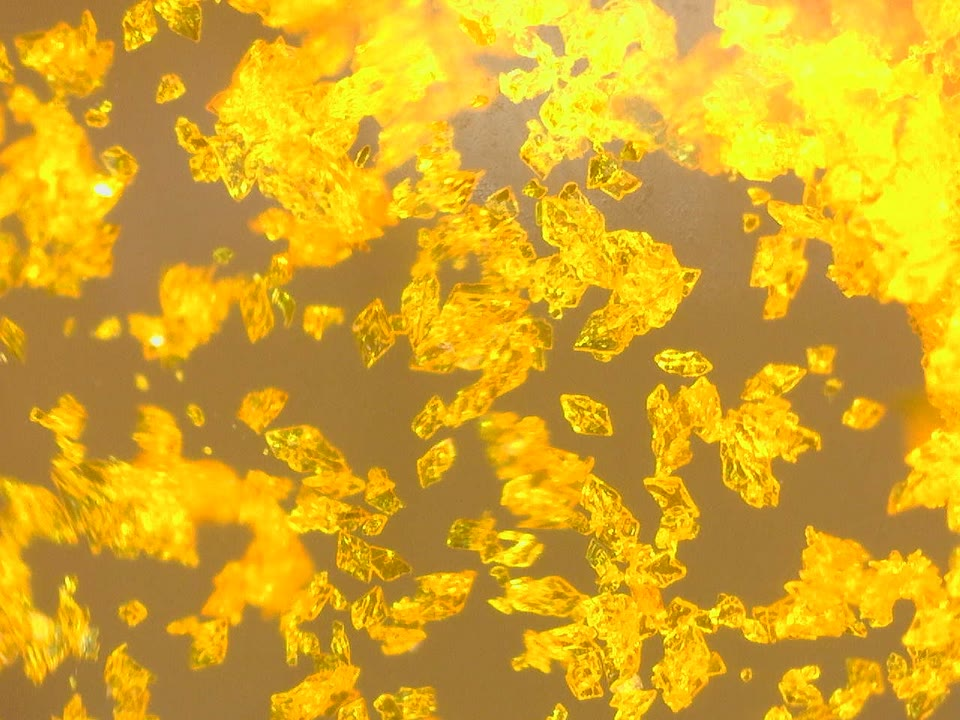
\includegraphics[width=0.5\linewidth]{images/book4/ferrocene-crystals.jpg}

{\small Crystals of ferrocene, $\ce{Fe(C5H5)2}$: an orange organometallic compound
stable in air, that sublimes on gentle warming.}
\end{omfigure}

\section{Electron counting and oxidation states}

\begin{method}[Counting electrons, two ways]\label{met:b3:organometallic-bonding:count}
\begin{enumerate}
  \item Neutral-ligand (covalent) method: the metal brings its group number of
        electrons; each ligand, taken neutral, brings 1 (H, \ce{CH3}, Cl, the
        $\eta^1$-allyl) or 2 (CO, \ce{PR3}, alkene) or more ($\eta^5$-\ce{C5H5} 5, $\eta^6$-\ce{C6H6} 6); add one per
        metal--metal bond and correct for the overall charge.
  \item Ionic method: ligands such as H, \ce{CH3}, Cl, \ce{C5H5} are counted as anions (2, 2,
        2 and 6 electrons), and the metal as the cation $d^n$ that results; neutral ligands
        as before.
  \item Both give the same total; the ionic method also gives the oxidation state
        and the $d^n$ count.
\end{enumerate}
\end{method}

\begin{example}[Counting]\label{ex:b3:organometallic-bonding:count}
$\ce{Fe(CO)5}$: $8 + 5 \times 2 = 18$, iron(0), $d^8$. Ferrocene: neutral method $8 + 2 \times 5 = 18$; ionic method
$\ce{Fe^{2+}}$ ($d^6$, 6) $+ 2 \times 6$ ($\ce{C5H5-}$) $= 18$, iron(II). $\ce{Mn2(CO)10}$: each Mn $7 + 5 \times 2 + 1$ (the Mn--Mn
bond) $= 18$. Square-planar $d^8$ complexes such as $\ce{[PtCl4]^{2-}}$ or Wilkinson's catalyst
$\ce{RhCl(PPh3)3}$ have 16 electrons: their empty $p_z$-like orbital is too high to fill, and
16-electron square-planar complexes are as stable as 18-electron ones.
\end{example}

\section{Carbonyls and phosphines}

\begin{definition}[Metal carbonyls]\label{def:b3:organometallic-bonding:carbonyl}
A \emph{metal carbonyl}\index{metal carbonyl} is a complex with carbon monoxide
ligands. A \emph{terminal carbonyl}\index{terminal carbonyl} is bonded to one
metal through carbon; a \emph{bridging carbonyl}\index{bridging carbonyl} spans
two (or three) metals.
\end{definition}

Ludwig Mond found in 1890 that nickel reacts with carbon monoxide at ordinary
temperature to give the volatile liquid $\ce{Ni(CO)4}$, which decomposes back to pure
nickel on heating: the basis of a refining process. Carbon monoxide binds
transition metals through its highest occupied orbital, a $\sigma$ lone pair mostly
on carbon, and accepts electrons into its empty $\pi^*$ orbitals, also larger on
carbon.

\begin{definition}[Synergic bonding]\label{def:b3:organometallic-bonding:synergic}
\emph{Synergic bonding}\index{synergic bonding} is the mutual reinforcement of
$\sigma$ donation from a ligand to a metal and $\pi$ back-donation from the metal to the
ligand: donation makes the metal richer in electrons and readier to give them
back, back-donation relieves the charge built up by donation.
\end{definition}

\begin{omfigure}
\begin{tikzpicture}[font=\small, >=Stealth]
  % sigma donation
  \fill[black!70] (0,0) circle (0.14); \node[anchor=north] at (0,-0.4) {M};
  \pic at (0,0) {omlobe={-0.7}{180}};
  \pic at (0,0) {omlobe={0.9}{0}};
  \node[circle, fill=black!40, inner sep=1.6pt] at (1.9,0) {};
  \node[circle, fill=omThm!70, inner sep=1.6pt] at (3.0,0) {};
  \pic at (1.9,0) {omlobe={0.85}{180}};
  \node[font=\scriptsize, anchor=north] at (1.9,-0.25) {C};
  \node[font=\scriptsize, anchor=north] at (3.0,-0.25) {O};
  \draw[->, thick, omThm] (1.4,0.55) to[bend right=30] (0.6,0.55);
  \node[anchor=north] at (1.5,-1.55) {$\sigma$ donation};
  % pi back-donation
  \begin{scope}[xshift=6.0cm]
    \fill[black!70] (0,0) circle (0.14); \node[anchor=north] at (0,-1.1) {M};
    \pic at (0,0) {omdxz};
    \node[circle, fill=black!40, inner sep=1.6pt] at (1.9,0) {};
    \node[circle, fill=omThm!70, inner sep=1.6pt] at (3.0,0) {};
    \pic at (1.9,0) {omp={0.9}{90}};
    \pic at (3.0,0) {omp={-0.6}{90}};
    \draw[->, thick, omThm] (0.6,1.05) to[bend left=30] (1.6,1.05);
    \node[anchor=north] at (1.5,-1.55) {$\pi$ back-donation};
  \end{scope}
\end{tikzpicture}

{\small \omterm{def:b3:organometallic-bonding:synergic}{Synergic bonding} of carbon monoxide. Left: the carbon lone pair ($\sigma$
orbital) donates into an empty $\sigma$-type metal orbital. Right: a filled metal $d$
orbital ($d_{xz}$, with its two axes) overlaps the empty $\pi^*$ orbital of CO, larger on
carbon, whose lobes match its phases: electrons flow back into an orbital that is
antibonding between C and O.}
\end{omfigure}

\begin{proposition}[CO stretching frequencies]\label{prop:b3:organometallic-bonding:co-frequency}
The more a metal back-donates into the $\pi^*$ orbitals of a CO ligand, the lower the
C--O stretching wavenumber.
\end{proposition}

\begin{proof}[Argued]
The $\pi^*$ orbitals of CO are antibonding between C and O: populating them weakens the
C--O bond, lowers its \omterm{def:b3:quantum-model-systems:oscillator}{force constant}, and hence the stretching wavenumber, which
varies as the square root of the \omterm{def:b3:quantum-model-systems:oscillator}{force constant} (\cref{ch:b3:rovibrational-spectroscopy}).
$\sigma$ donation removes electrons from an orbital nearly non-bonding (slightly
antibonding) for C--O, which by itself would raise the wavenumber a little: the
observed decrease shows that back-donation dominates.
\end{proof}

Free carbon monoxide has its fundamental at $\omega_e - 2\omega_ex_e = \qty{2143}{cm^{-1}}$; \omterm{def:b3:organometallic-bonding:carbonyl}{terminal
carbonyls} of neutral complexes absorb roughly between 1900 and \qty{2100}{cm^{-1}},
\omterm{def:b3:organometallic-bonding:carbonyl}{bridging carbonyls} lower still. Along an isoelectronic series, an anionic
carbonyl absorbs at lower wavenumber than the neutral one, a cationic one at
higher: the more electron-rich the metal, the more it back-donates. The number of
bands, from symmetry (\cref{ch:b3:group-theory-applied}), gives the geometry.
% ledger: diat:CO.we, diat:CO.wexe

\begin{proposition}[$\pi$ interactions and the ligand-field splitting]\label{prop:b3:organometallic-bonding:pi-delta}
In an octahedral complex, $\pi$-acceptor ligands increase $\Delta_{\mathrm o}$ and $\pi$-donor ligands
decrease it.
\end{proposition}

\begin{proof}
The $e_g$ orbitals have $\sigma$ symmetry only. The $t_{2g}$ orbitals ($d_{xy}$, $d_{xz}$, $d_{yz}$) match a $t_{2g}$
combination of ligand $\pi$ orbitals: for $d_{xy}$, the four ligands in the $xy$ plane each
offer a $\pi$ orbital perpendicular to their M--L axis in that plane, and the
combination with alternating signs has the symmetry of $d_{xy}$ (the remaining
combinations transform as $t_{1g}$, $t_{1u}$ and $t_{2u}$ and find no $d$ partner). Two orbitals of
the same symmetry mix and repel: the lower is pushed down, the upper up. A
$\pi$ acceptor offers empty orbitals above the $t_{2g}$ set, which is pushed down: $\Delta_{\mathrm o}$
increases. A $\pi$ donor offers filled orbitals below it, which push it up: $\Delta_{\mathrm o}$
decreases. The $e_g$ level is unaffected in both cases.
\end{proof}

This is why CO and \ce{CN-} sit at the strong end of the spectrochemical series, and
halides and hydroxide at the weak end, as the Year 2 volume stated.

\begin{definition}[Tolman parameters]\label{def:b3:organometallic-bonding:tolman}
The \emph{Tolman cone angle}\index{Tolman cone angle} of a phosphine is the apex
angle of the cone, centred on the metal at a standard distance, that just
encloses the van der Waals surfaces of its substituents: a measure of its size.
The \emph{Tolman electronic parameter}\index{Tolman electronic parameter} is the
wavenumber of the symmetric CO stretch of $\ce{Ni(CO)3L}$: the more strongly the
phosphine L donates, the lower it is.
\end{definition}

Phosphines are tuned independently in size and electron donation by their
substituents: trialkylphosphines are stronger donors than triarylphosphines,
phosphites the weakest; $\ce{P(tBu)3}$ is far bulkier than $\ce{PMe3}$. Bulky phosphines favour
low coordination numbers and fast ligand dissociation, which is why they
appear in so many catalysts.

\section{$\pi$ ligands}

\begin{definition}[Dewar--Chatt--Duncanson model]\label{def:b3:organometallic-bonding:dcd}
The \emph{Dewar--Chatt--Duncanson model}\index{Dewar--Chatt--Duncanson model} of
the bonding of an alkene to a metal combines $\sigma$ donation from the C=C $\pi$ orbital
to an empty metal orbital with back-donation from a filled metal $d$ orbital into
the C=C $\pi^*$ orbital. Its limit of strong back-donation is a
\emph{metallacyclopropane}\index{metallacyclopropane}, a three-membered ring
with two M--C $\sigma$ bonds and a C--C single bond.
\end{definition}

\begin{proposition}[Consequences of back-donation to an alkene]\label{prop:b3:organometallic-bonding:dcd}
Coordination lengthens the C=C bond and bends the substituents back, away from
the metal, more so as back-donation increases.
\end{proposition}

\begin{proof}[Argued]
Removing electrons from the $\pi$ (bonding) orbital and adding them to the $\pi^*$
(antibonding) orbital both lower the C--C bond order. Mixing $\pi^*$ character
rehybridises the carbons towards $sp^3$, whose bonds to the substituents point away
from the metal, towards the \omterm{def:b3:organometallic-bonding:dcd}{metallacyclopropane} geometry.
\end{proof}

\begin{omfigure}
\begin{tikzpicture}[font=\small, >=Stealth]
  \fill[black!70] (0,0) circle (0.14); \node[anchor=north] at (0,-1.1) {M};
  \pic at (0,0) {omlobe={0.9}{0}};
  \foreach \y in {0.45,-0.45}{\node[circle, fill=black!40, inner sep=1.6pt] at (1.9,\y) {};}
  \pic at (1.9,0.45) {omp={-0.75}{0}};
  \pic at (1.9,-0.45) {omp={-0.75}{0}};
  \draw[->, thick, omThm] (1.3,1.0) to[bend right=30] (0.5,0.6);
  \node[anchor=north] at (1.2,-1.4) {$\sigma$: $\pi$(C=C) $\to$ M};
  \begin{scope}[xshift=5.6cm]
    \fill[black!70] (0,0) circle (0.14); \node[anchor=north] at (0,-1.1) {M};
    \pic at (0,0) {omdxy};
    \foreach \y in {0.45,-0.45}{\node[circle, fill=black!40, inner sep=1.6pt] at (1.9,\y) {};}
    \pic at (1.9,0.45) {omp={-0.75}{0}};
    \pic at (1.9,-0.45) {omp={0.75}{0}};
    \draw[->, thick, omThm] (0.7,0.9) to[bend left=30] (1.5,0.9);
    \node[anchor=north] at (1.2,-1.4) {$\pi$: M $\to$ $\pi^*$(C=C)};
  \end{scope}
\end{tikzpicture}

{\small The \omterm{def:b3:organometallic-bonding:dcd}{Dewar--Chatt--Duncanson model} of an alkene bound side-on (C=C
vertical, the metal on the left). Left: the filled $\pi$ orbital (two $p$ orbitals in
phase) donates into an empty metal orbital. Right: a filled metal $d$ orbital
of matching phases donates into the empty $\pi^*$ orbital (the two $p$ orbitals out of
phase).}
\end{omfigure}

Zeise's salt, $\ce{K[PtCl3(C2H4)]}$, made in 1827, was the first organometallic compound
of a transition metal; its ethene lies perpendicular to the \ce{PtCl3} plane, as
the model predicts. Allyl ($\eta^3$), dienes ($\eta^4$), arenes ($\eta^6$) and the cyclopentadienyl
ring ($\eta^5$) bind in the same way through several carbons at once.

\begin{definition}[Metallocenes]\label{def:b3:organometallic-bonding:metallocene}
A \emph{sandwich compound}\index{sandwich compound} has a metal between two
parallel planar ring ligands bonded through all their carbons; a
\emph{metallocene}\index{metallocene} is a sandwich compound with two $\eta^5$-cyclopentadienyl
rings, $\ce{M(C5H5)2}$.
\end{definition}

\begin{proposition}[The frontier orbitals of ferrocene]\label{prop:b3:organometallic-bonding:ferrocene}
In a \omterm{def:b3:organometallic-bonding:metallocene}{metallocene} with parallel rings ($D_{5d}$), the metal $d$ orbitals split into $e_{2g}$
($d_{xy}$, $d_{x^2-y^2}$) and $a_{1g}$ ($d_{z^2}$), nearly non-bonding and close together, and $e_{1g}^\ast$ ($d_{xz}$,
$d_{yz}$), strongly antibonding; ferrocene, with six $d$ electrons in $e_{2g}^4a_{1g}^2$, has 18
electrons and no unpaired electron.
\end{proposition}

\begin{proof}[Argued]
The $\pi$ orbitals of the two rings combine into symmetry-adapted pairs $a_{1g}$, $a_{2u}$,
$e_{1g}$, $e_{1u}$, $e_{2g}$, $e_{2u}$ (from the five $\pi$ orbitals of each ring, with zero, one and two
nodal planes through the axis). The filled ring $e_{1g}$ combination overlaps
strongly with $d_{xz}$, $d_{yz}$ (one nodal plane through the axis each): they form bonding
orbitals, mostly ring, and antibonding $e_{1g}^\ast$, mostly metal, pushed high. $d_{xy}$, $d_{x^2-y^2}$
(two nodal planes) meet only the empty ring $e_{2g}$ orbitals and are slightly
stabilised by back-donation; $d_{z^2}$ points at the hole in the middle of each ring and
hardly overlaps. Six electrons fill $e_{2g}$ and $a_{1g}$; with the twelve electrons of the
bonding ring combinations, the count is 18.
\end{proof}

\begin{omfigure}
\begin{tikzpicture}[font=\small]
  % sandwich drawing
  \begin{scope}[xshift=-1.0cm]
    \draw[thick, fill=black!8] (0,1.0) ellipse (1.0 and 0.3);
    \draw[thick, fill=black!8] (0,-1.0) ellipse (1.0 and 0.3);
    \foreach \a in {90,162,234,306,18}{\fill[black!60] ({cos(\a)},{1.0+0.3*sin(\a)}) circle (0.07);
      \fill[black!60] ({cos(\a)},{-1.0+0.3*sin(\a)}) circle (0.07);}
    \shade[ball color=orange!70!brown] (0,0) circle (0.2);
    \node[anchor=west] at (0.25,0) {Fe};
  \end{scope}
  % level diagram for four metallocenes
  \pic[transform shape] at (2.1,-0.9) {omlevel={u}{0.5}};
  \pic[transform shape] at (2.7,-0.9) {omlevel={ud}{0.5}};
  \pic[transform shape] at (2.4,-0.4) {omlevel={ud}{0.5}};
  \pic[transform shape] at (2.1,1.0) {omlevel={}{0.5}};
  \pic[transform shape] at (2.7,1.0) {omlevel={}{0.5}};
  \node[anchor=north] at (2.4,-1.3) {\ce{[FeCp2]+}};
  \node[anchor=north, font=\scriptsize] at (2.4,-1.75) {17 e$^-$};
  \pic[transform shape] at (4.3,-0.9) {omlevel={ud}{0.5}};
  \pic[transform shape] at (4.9,-0.9) {omlevel={ud}{0.5}};
  \pic[transform shape] at (4.6,-0.4) {omlevel={ud}{0.5}};
  \pic[transform shape] at (4.3,1.0) {omlevel={}{0.5}};
  \pic[transform shape] at (4.9,1.0) {omlevel={}{0.5}};
  \node[anchor=north] at (4.6,-1.3) {\ce{FeCp2}};
  \node[anchor=north, font=\scriptsize] at (4.6,-1.75) {18 e$^-$};
  \pic[transform shape] at (6.5,-0.9) {omlevel={ud}{0.5}};
  \pic[transform shape] at (7.1,-0.9) {omlevel={ud}{0.5}};
  \pic[transform shape] at (6.8,-0.4) {omlevel={ud}{0.5}};
  \pic[transform shape] at (6.5,1.0) {omlevel={u}{0.5}};
  \pic[transform shape] at (7.1,1.0) {omlevel={}{0.5}};
  \node[anchor=north] at (6.8,-1.3) {\ce{CoCp2}};
  \node[anchor=north, font=\scriptsize] at (6.8,-1.75) {19 e$^-$};
  \pic[transform shape] at (8.7,-0.9) {omlevel={ud}{0.5}};
  \pic[transform shape] at (9.3,-0.9) {omlevel={ud}{0.5}};
  \pic[transform shape] at (9.0,-0.4) {omlevel={ud}{0.5}};
  \pic[transform shape] at (8.7,1.0) {omlevel={u}{0.5}};
  \pic[transform shape] at (9.3,1.0) {omlevel={u}{0.5}};
  \node[anchor=north] at (9.0,-1.3) {\ce{NiCp2}};
  \node[anchor=north, font=\scriptsize] at (9.0,-1.75) {20 e$^-$};
  \node[anchor=east, font=\scriptsize] at (1.8,-0.9) {$e_{2g}$};
  \node[anchor=east, font=\scriptsize] at (1.8,-0.4) {$a_{1g}$};
  \node[anchor=east, font=\scriptsize] at (1.8,1.0) {$e_{1g}^\ast$};
\end{tikzpicture}

{\small Left: the sandwich structure of ferrocene (eclipsed rings). Right: the
$d$-based frontier orbitals of \omterm{def:b3:organometallic-bonding:metallocene}{metallocenes}, $e_{2g}$ and $a_{1g}$ nearly non-bonding, $e_{1g}^\ast$
antibonding, filled for the ferrocenium cation (17 electrons), ferrocene (18),
cobaltocene (19) and nickelocene (20, one electron in each $e_{1g}^\ast$ orbital, spins
parallel by Hund's rule).}
\end{omfigure}

\section{Carbenes, carbynes and metal--metal bonds}

\begin{definition}[Carbenes and carbene complexes]\label{def:b3:organometallic-bonding:carbene}
A \emph{carbene}\index{carbene} is a neutral species $\ce{R2C}$ with a divalent carbon
carrying two non-bonding electrons. A \emph{carbene complex}\index{carbene complex}
has a $\ce{CR2}$ ligand bonded to a metal by a double bond, $\ce{M=CR2}$. A
\emph{Fischer carbene}\index{Fischer carbene} complex has a heteroatom substituent
on the carbene carbon and a low-valent metal with $\pi$-acceptor ligands; its carbene
carbon is electrophilic. A \emph{Schrock carbene}\index{Schrock carbene} (alkylidene)
complex has only C or H substituents and a high-valent early metal; its carbon is
nucleophilic. An \emph{N-heterocyclic carbene}\index{N-heterocyclic carbene} is a
cyclic carbene flanked by two nitrogen atoms, stable as a free compound and a strong
$\sigma$-donor ligand.
\end{definition}

The two kinds of \omterm{def:b3:organometallic-bonding:carbene}{carbene complexes} differ in the way the M=C bond is shared.
In a \omterm{def:b3:organometallic-bonding:carbene}{Fischer carbene} a singlet \omterm{def:b3:organometallic-bonding:carbene}{carbene} donates its lone pair to the metal and
receives back-donation into its empty $p$ orbital, which the heteroatom lone pair
also stabilises: the carbon stays electron-poor, attacked by nucleophiles. In a
\omterm{def:b3:organometallic-bonding:carbene}{Schrock carbene} two triplet fragments, metal and \omterm{def:b3:organometallic-bonding:carbene}{carbene}, form a covalent $\sigma +
\pi$ bond, polarised towards carbon: the alkylidene behaves like a Wittig ylide.

\begin{definition}[Carbyne complex]\label{def:b3:organometallic-bonding:carbyne}
A \emph{carbyne complex}\index{carbyne complex} has a triple bond between a metal
and a carbon carrying one substituent, $\ce{M#CR}$.
\end{definition}

\begin{definition}[$\delta$ bond, quadruple bond]\label{def:b3:organometallic-bonding:delta}
A \emph{$\delta$ bond}\index{delta bond@$\delta$ bond} is a bond whose orbital has two nodal planes
containing the internuclear axis, formed by the face-to-face overlap of two $d$
orbitals such as $d_{xy}$ and $d_{xy}$. A \emph{quadruple bond}\index{quadruple bond}
combines one $\sigma$, two $\pi$ and one $\delta$ bond between two metal atoms.
\end{definition}

\begin{proposition}[{The \omterm{def:b3:organometallic-bonding:delta}{quadruple bond} of $[\mathrm{Re_2Cl_8}]^{2-}$}]\label{prop:b3:organometallic-bonding:quadruple}
In $\ce{[Re2Cl8]^{2-}}$ (two \ce{Re^{III}}, $d^4$ each), the eight $d$ electrons occupy $\sigma^2\pi^4\delta^2$: a bond
order of 4, which requires the eclipsed arrangement of the two \ce{ReCl4} units.
\end{proposition}

\begin{proof}
With $z$ along the Re--Re axis and the Cl atoms along $\pm x$ and $\pm y$ on each Re, $d_{x^2-y^2}$
points at the chlorides and is used in Re--Cl bonding. The other four $d$ orbitals
of each metal overlap pairwise: $d_{z^2}$ with $d_{z^2}$ along the axis ($\sigma$), $d_{xz}$ with $d_{xz}$ and $d_{yz}$
with $d_{yz}$ side by side ($\pi$, twice), $d_{xy}$ with $d_{xy}$ face to face ($\delta$, the weakest).
Eight electrons fill the four bonding combinations. Rotating one unit by $45^\circ$
about $z$ turns its $d_{xy}$ into $d_{x^2-y^2}$, which has zero overlap with the other $d_{xy}$ by
symmetry: the $\delta$ bond, and with it the eclipsed preference, is lost. The
other three overlaps are cylindrically symmetric or unchanged in magnitude.
\end{proof}

% ledger: geom:Re2Cl8.ReRe
The Re--Re distance of \qty{2.24}{\angstrom} in the potassium salt is very short for two metal atoms, and the chlorides of the two halves are indeed eclipsed, against
their steric repulsion: the $\delta$ bond, weak as it is, holds them there.

\begin{omfigure}
\tdplotsetmaincoords{58}{25}
\begin{tikzpicture}[tdplot_main_coords, font=\small, scale=1.15]
  \draw[thick, black!60] (0,0,0) -- (0,0,2.0);
  \foreach \z in {0,2.0}{
    \foreach \b in {0,90,180,270}{
      \draw[black!45] (0,0,\z) -- ({1.55*cos(\b)},{1.55*sin(\b)},\z);}
    \foreach \a/\s in {45/omphasepos, 135/omphaseneg, 225/omphasepos, 315/omphaseneg}{
      \path[\s, opacity=0.9] plot[domain=0:360, samples=48, smooth cycle]
        ({0.62*cos(\a)+0.55*cos(\x)*cos(\a)-0.26*sin(\x)*sin(\a)},
         {0.62*sin(\a)+0.55*cos(\x)*sin(\a)+0.26*sin(\x)*cos(\a)}, {\z});}
    \foreach \b in {0,90,180,270}{
      \node[circle, fill=green!45!black, inner sep=1.8pt] at ({1.55*cos(\b)},{1.55*sin(\b)},\z) {};}
    \shade[ball color=black!40] (0,0,\z) circle (0.14);}
  \node[anchor=east, xshift=-1.9cm] at (0,0,2.0) {Re};
  \node[anchor=east, xshift=-1.9cm] at (0,0,0) {Re};
\end{tikzpicture}

{\small The $\delta$ component of the \omterm{def:b3:organometallic-bonding:delta}{quadruple bond} of $\ce{[Re2Cl8]^{2-}}$: the $d_{xy}$ orbitals of
the two rhenium atoms (four lobes each, signs blue and orange) face each other
across the Re--Re axis, lobe over lobe of the same sign. The chlorides (green),
eclipsed, lie along $x$ and $y$, between the lobes.}
\end{omfigure}

\section{The isolobal analogy}

\begin{definition}[Isolobal fragments]\label{def:b3:organometallic-bonding:isolobal}
Two molecular fragments are \emph{isolobal}\index{isolobal fragments} when the
number, symmetry, approximate energy and shape of their frontier orbitals, and the
number of electrons in them, are similar. The \emph{isolobal
analogy}\index{isolobal analogy} predicts that isolobal fragments can replace one
another in molecules.
\end{definition}

\begin{proposition}[Isolobal series]\label{prop:b3:organometallic-bonding:isolobal}
$\ce{CH3}$, $\ce{Mn(CO)5}$ and $\ce{CpFe(CO)2}$ are \omterm{def:b3:organometallic-bonding:isolobal}{isolobal} (one frontier orbital, one electron);
$\ce{CH2}$ and $\ce{Fe(CO)4}$ (two orbitals, two electrons); $\ce{CH}$ and $\ce{Co(CO)3}$ (three orbitals,
three electrons).
\end{proposition}

\begin{proof}[Argued]
$\ce{CH3}$ is a tetrahedral fragment missing one bond: one $sp^3$-like orbital with one
electron, one short of an octet. $\ce{Mn(CO)5}$ is an octahedron missing one ligand: the
empty site holds one hybrid orbital pointing out; with $7 + 10 = 17$ electrons it is one
short of 18, and its single electron sits in that hybrid. Removing two or three
ligands (or bonds) gives two or three such orbitals and electrons, with the
same counting on both sides: $\ce{Fe(CO)4}$ has 16 electrons ($8 + 8$), two short of 18;
$\ce{Co(CO)3}$ has 15 ($9 + 6$), three short.
\end{proof}

\begin{method}[Predicting a structure by isolobal replacement]\label{met:b3:organometallic-bonding:isolobal}
\begin{enumerate}
  \item Break the compound into fragments and count each one's frontier orbitals
        and electrons.
  \item Replace each fragment by its organic \omterm{def:b3:organometallic-bonding:isolobal}{isolobal} partner.
  \item The organic analogue, if it exists, suggests the bonding and the shape:
        $\ce{Mn2(CO)10}$ is ``ethane'', $\ce{Co3(CO)9CH}$ is ``tetrahedrane'' $\ce{(CH)4}$ with three CH
        replaced by $\ce{Co(CO)3}$.
\end{enumerate}
\end{method}

\begin{omfigure}
\begin{tikzpicture}[font=\small]
  \foreach \y/\l/\r/\n in {0/{\ce{CH3}}/{\ce{Mn(CO)5}}/1, -1.6/{\ce{CH2}}/{\ce{Fe(CO)4}}/2, -3.2/{\ce{CH}}/{\ce{Co(CO)3}}/3}{
    \node at (0,\y) {\l};
    \node at (5.2,\y) {\r};
    \node[font=\large] at (2.6,\y) {$\longleftrightarrow$};
    \node[font=\scriptsize, anchor=south] at (2.6,\y+0.15) {isolobal};
    \node[font=\scriptsize, anchor=west] at (7.0,\y) {\ifnum\n=1 one frontier orbital, one electron\else\ifnum\n=2 two frontier orbitals, two electrons\else three frontier orbitals, three electrons\fi\fi};}
  \foreach \a in {0}{\pic at (0.55,0) {omlobe={0.6}{0}};}
  \pic at (6.25,0) {omlobe={0.6}{0}};
  \pic at (0.45,-1.6) {omlobe={0.6}{20}}; \pic at (0.45,-1.6) {omlobe={0.6}{-20}};
  \pic at (6.15,-1.6) {omlobe={0.6}{20}}; \pic at (6.15,-1.6) {omlobe={0.6}{-20}};
  \foreach \t in {-30,0,30}{\pic at (0.4,-3.2) {omlobe={0.55}{\t}}; \pic at (6.1,-3.2) {omlobe={0.55}{\t}};}
\end{tikzpicture}

{\small The \omterm{def:b3:organometallic-bonding:isolobal}{isolobal} series (frontier hybrids drawn schematically): each organic
fragment and the \omterm{def:b3:organometallic-bonding:carbonyl}{metal carbonyl} fragment opposite it have the same number of
outward-pointing frontier orbitals and of electrons in them, and combine in
analogous ways.}
\end{omfigure}

\begin{definition}[Agostic interaction]\label{def:b3:organometallic-bonding:agostic}
An \emph{agostic interaction}\index{agostic interaction} is a three-centre,
two-electron bond between a metal and a C--H bond of one of its own ligands, in
which the C--H bonding pair donates into an empty metal orbital.
\end{definition}

Agostic hydrogens show up as short metal--hydrogen distances in diffraction
structures, as unusually low C--H stretching wavenumbers, and in NMR as a
high-field shift and a reduced $^1J_{\mathrm{CH}}$ coupling. They are frozen snapshots of
C--H activation, the first step of many catalytic reactions.

\begin{inthelab}[Working with metal carbonyls]
\omterm{def:b3:organometallic-bonding:carbonyl}{Metal carbonyls} are handled in a fume hood with a working extraction, under
nitrogen or argon, with no open flame: many release carbon monoxide on
warming. Volatile carbonyls are transferred by cannula or on a vacuum line, never
poured; residues are destroyed by slow oxidation (bleach or bromine water) in the
hood. Nickel tetracarbonyl, the most dangerous, is not used in teaching
laboratories at all.
\end{inthelab}

\begin{safety}{\ghs[0.62cm]{GHS02}\ghs[0.62cm]{GHS06}\ghs[0.62cm]{GHS07}\ghs[0.62cm]{GHS08}\ghs[0.62cm]{GHS09}}
% ledger: ghs4:NiCO4, ghs4:ferrocene
Nickel tetracarbonyl: highly flammable, fatal if inhaled, suspected carcinogen,
may damage the unborn child. Ferrocene: a flammable solid, harmful if swallowed;
handled as a fine chemical with gloves and dust precautions.
\end{safety}

\begin{history}[Mond's carbonyl and the sandwich]
Ludwig Mond and his co-workers discovered nickel tetracarbonyl in 1890 while
studying the corrosion of nickel valves by carbon monoxide, and built on it a
process for refining nickel. Ferrocene was made in 1951 by Thomas Kealy and Peter
Pauson, and independently by Samuel Miller, John Tebboth and John Tremaine; in 1952
Geoffrey Wilkinson and Robert Woodward, and Ernst Otto Fischer, proposed the
sandwich structure. Fischer and Wilkinson shared the 1973 Nobel Prize in
Chemistry for their work on \omterm{def:b3:organometallic-bonding:metallocene}{sandwich compounds}.
\end{history}

\section{Exercises}

\begin{exercise}[$\star$]\label{exo:b3:organometallic-bonding:1}
Count the valence electrons of $\ce{Fe(CO)5}$, $\ce{Mn2(CO)10}$ (per Mn), $\ce{CpMo(CO)3H}$, Zeise's anion
$\ce{[PtCl3(C2H4)]-}$, $\ce{Cr($\eta^6$-C6H6)(CO)3}$ and $\ce{Cp2ZrCl2}$.
\end{exercise}

\begin{exercise}[$\star$]\label{exo:b3:organometallic-bonding:2}
Give the oxidation state and $d^n$ count of the metal in each compound of the
previous exercise.
\end{exercise}

\begin{exercise}[$\star$]\label{exo:b3:organometallic-bonding:3}
Rank the CO stretching wavenumbers of $\ce{[V(CO)6]-}$, $\ce{Cr(CO)6}$ and $\ce{[Mn(CO)6]+}$, and justify.
\end{exercise}

\begin{exercise}[$\star$]\label{exo:b3:organometallic-bonding:4}
Give the organic \omterm{def:b3:organometallic-bonding:isolobal}{isolobal} analogues of $\ce{Mn2(CO)10}$, $\ce{[CpFe(CO)2]2}$ and $\ce{Co3(CO)9CH}$.
\end{exercise}

\begin{exercise}[$\star\star$]\label{exo:b3:organometallic-bonding:5}
How many CO stretching bands do $fac$- and $mer$-$\ce{M(CO)3L3}$ show in the IR?
\end{exercise}

\begin{exercise}[$\star\star$]\label{exo:b3:organometallic-bonding:6}
Explain why replacing $\ce{PMe3}$ by $\ce{P(tBu)3}$ in a catalyst can speed up a step that needs a
ligand to leave the metal.
\end{exercise}

\begin{exercise}[$\star\star$]\label{exo:b3:organometallic-bonding:7}
Classify $\ce{(CO)5Cr=C(OMe)Ph}$ and $\ce{Ta(=CHCMe3)(CH2CMe3)3}$ as Fischer or Schrock \omterm{def:b3:organometallic-bonding:carbene}{carbene
complexes}, and predict their reactions with an amine and with a ketone.
\end{exercise}

\begin{exercise}[$\star\star$]\label{exo:b3:organometallic-bonding:8}
What bond order would a staggered $\ce{[Re2Cl8]^{2-}}$ have? What is the bond order of
$\ce{[Re2Cl8]^{4-}}$, with two more electrons?
\end{exercise}

\begin{exercise}[$\star\star$]\label{exo:b3:organometallic-bonding:9}
List three kinds of evidence for an agostic C--H interaction.
\end{exercise}

\begin{exercise}[$\star\star\star$]\label{exo:b3:organometallic-bonding:10}
Give examples of stable complexes with 16, 17 and 19 valence electrons, and explain
each exception to the 18-electron rule.
\end{exercise}

\begin{exercise}[$\star\star\star$]\label{exo:b3:organometallic-bonding:11}
$\ce{Cr(CO)6}$ is colourless and diamagnetic. Explain, using the $\pi$-acceptor effect on $\Delta_{\mathrm o}$,
why it is low spin and why its $d$--$d$ bands lie in the ultraviolet.
\end{exercise}

\begin{exercise}[$\star\star\star$]\label{exo:b3:organometallic-bonding:12}
The C--C bond of ethene lengthens from \qty{1.34}{\angstrom} to \qty{1.37}{\angstrom} in Zeise's salt and to
about \qty{1.43}{\angstrom} in a complex of a low-valent metal with strong back-donation (data of the
exercise). Interpret with the \omterm{def:b3:organometallic-bonding:dcd}{Dewar--Chatt--Duncanson model}.
\end{exercise}

\section{Problem: Sandwiches}

\begin{problem}[{Weekend problem --- sandwiches: electron counts of four
metallocenes, their frontier orbitals and unpaired electrons, their redox
chemistry, and two isolobal and spectroscopic questions}]
\label{pb:b3:organometallic-bonding:1}
\omterm{def:b3:organometallic-bonding:metallocene}{Metallocenes} $\ce{MCp2}$ ($\ce{Cp} = \eta^5$-$\ce{C5H5}$) are known for M = Fe, Co, Ni and for the ferrocenium cation.

\medskip\noindent\textbf{Part I --- Counting.}
\begin{enumerate}
  \item Count the electrons of ferrocene by the ionic method.
  \item Count them by the neutral method.
  \item Count cobaltocene.
  \item Count nickelocene.
  \item Count the ferrocenium cation.
  \item Give the oxidation state and $d^n$ count of each metal.
\end{enumerate}

\medskip\noindent\textbf{Part II --- Orbitals and magnetism.}
\begin{enumerate}[resume]
  \item Classify the five $d$ orbitals in $D_{5d}$.
  \item Which of them overlap strongly with the ring $\pi$ orbitals, and with what
        consequence?
  \item Give the order of the $d$-based levels.
  \item Fill them for ferrocene: unpaired electrons?
  \item Fill them for cobaltocene: unpaired electrons and \omterm{def:b3:complex-spectra-magnetism:moment}{spin-only moment}?
  \item Fill them for nickelocene: unpaired electrons and \omterm{def:b3:complex-spectra-magnetism:moment}{spin-only moment}?
  \item Fill them for ferrocenium: unpaired electrons? Why is its measured moment
        above the spin-only value?
\end{enumerate}

\medskip\noindent\textbf{Part III --- Redox.}
\begin{enumerate}[resume]
  \item Why is cobaltocene a strong reducing agent?
  \item Why is the ferrocene/ferrocenium couple fast and reversible?
  \item Why is it used as an internal reference in non-aqueous electrochemistry
        (\cref{ch:b3:electrode-kinetics})?
  \item What would you expect of nickelocene's reactions with two-electron
        ligands?
\end{enumerate}

\medskip\noindent\textbf{Part IV --- Fragments and spectra.}
\begin{enumerate}[resume]
  \item Show that $\ce{CpFe(CO)2}$ is \omterm{def:b3:organometallic-bonding:isolobal}{isolobal} with \ce{CH3}, and predict the structure of
        $\ce{[CpFe(CO)2]2}$.
  \item What mixed dimer could it form with $\ce{Mn(CO)5}$?
  \item How does replacing a CO of $\ce{CpMn(CO)3}$ by $\ce{PPh3}$ change the remaining CO
        stretches?
  \item How many CO bands does $\ce{Cr($\eta^6$-C6H6)(CO)3}$ ($C_{3v}$) show?
  \item Why can a $\eta^5$-Cp ring slip to $\eta^3$ during a substitution?
  \item State the result: the spin-only magnetic moment of nickelocene.
\end{enumerate}
\end{problem}
